\documentclass[11pt]{beamer}
\usetheme{AnnArbor}
\usepackage[utf8]{inputenc}
\usepackage[czech]{babel}
\usepackage{amsmath}
\usepackage{amsfonts}
\usepackage{amssymb}
\usepackage{graphicx}
\author{David Paleček,Matěj Lebeda, Veronika Funková, Martin Hrba}
\title{Distribution of players into teams.}
%\setbeamercovered{transparent} 
%\setbeamertemplate{navigation symbols}{} 
%\logo{} 
%\institute{} 
%\date{} 
%\subject{} 


\begin{document}

\begin{frame}
\titlepage
\end{frame}

%\begin{frame}
%\tableofcontents
%\end{frame}

\begin{frame}{Optimization problem}
Community/ online tournaments:
\begin{itemize}
\item Players don´t know each other
\item Assigned role and known ranking of each player
\item 8/16/32/64/128 teams of 3/5/11 players
\end{itemize}
\vspace{1cm}
Goal: try to make the teams \uv{balanced}.
\end{frame}

\begin{frame}{Brute--forcing}
When each player has unique role in a team:\\\vspace{0.5 cm}
Total $(t!)^{\kappa-1}$ combinations of distributions, where t is number of teams and $\kappa$ number of roles\\\vspace{0.5cm}
for 16 teams, and 5 roles $\approx 2\cdot 10^{53}$ combinations.\\
\end{frame}
 
\begin{frame}{Variables}
\begin{itemize}
\item $I$ set of players\\
\item $T$ set of teams\\
\item $Roles$ set of roles $\kappa$
\item $x_{it}$ - binary variable, player i is in team t
\item $\kappa_i$ - role of i-th player
\item $n_{\kappa}$ number of players in team with role $\kappa$
\item $rank_i$ rank of i-th player
\end{itemize}
\end{frame}




\begin{frame}{Formulation of problem}
\begin{equation*}
\small
\begin{aligned}
\underset{x_it}{\text{min}} \sum_{t} s_t^{+} + s_t^{-}&\\
s.t.\quad \quad\quad \quad\quad\quad\quad \quad \sum_t x_{it} =1   \quad &\forall i \in I\\
\sum_i x_{it} =team\,size   \quad &\forall t \in T\\
\sum_i \mathbb{I}_{[\kappa_i=\kappa ]} x_{it} = n_{\kappa} \quad &\forall \kappa \in Roles, t \in T\\ 
\sum_i rank_i x_{it} + s_t^{-} - s_t^{+} = 5 \,\overline{rank} \quad &\forall t \in T \\
x_{it} \in \{0,1\} \quad &\forall i \in I, t\in T
\end{aligned}
\end{equation*}
\end{frame}

\begin{frame}
Rank of player can range from 100 to 3000\\\vspace{0.4cm}
Number of variables : $(|I|+2)*|T|$\\\vspace{0.4 cm}
Doubling number of players:
\begin{itemize}
\item quadruples number of variables
\item doubles number of constraints\vspace{0.4 cm}
\end{itemize}
1000 players in teams of 5 $\implies$ 200 400 variables
\end{frame}

\begin{frame}{Branch and Bound}
Variables aren´t treated as binary but as continuous.\\
In each layer fixes value of one variable.\\
Problem is quickly solved by simplex.\\
If it leads to at best unfeasible or "bad" solution, node is pruned. 
\begin{figure}
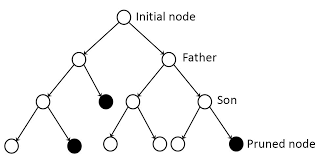
\includegraphics[width=8cm]{branch.png}
\caption{First layers of solving the problem.}
\end{figure}
\end{frame}

\begin{frame}{Paralel computing}
By using 64 nodes we can
\begin{itemize}
\item speed up matrix operations inside simplex.
\item or go to 8th layer and in parraler solve 64 \uv{subproblems} which can be cross-checked with left-over nodes redistributed.
\end{itemize}
\end{frame}

\begin{frame}{Speed $\&$ memory}
With 80 players in 16 teams \uv{good} solution is reached in 15 second on notebook.\\\vspace{0.5cm}

With hundrets of players memory could be ok, but speed???
\end{frame}
\end{document}
